
\documentclass[12pt,a4paper]{report}
\usepackage[utf8]{inputenc}
\usepackage{amsmath}
\usepackage{amsfonts}
\usepackage{amssymb}
\usepackage{graphicx}
\usepackage{enumitem}
\usepackage[left=2cm, right=2cm, top=4cm, bottom=2cm]{geometry}

\begin{document}
	%Portada
	\begin{titlepage}
		\centering
		{\scshape\LARGE Universidad Nacional Autónoma de México \par}
		\vspace{1cm}
		{\scshape\Large Probabilidad I\par}
		\vspace{1.5cm}
		{\huge\bfseries Tarea V\par}
		\vspace{.5cm}

		{\Large\itshape Alan Ernesto Arteaga Vázquez \par}
		 \vspace{.5cm}
		{\Large\itshape Raúl Llamosas Alvarado \par}
		 \vspace{.5cm}
		{\Large\itshape Edgar Quiroz Castañeda \par}
	    \vspace{.5cm}
		{\Large\itshape Jean Paul Ruiz Melo\par}
		\vspace{.5cm}
		{\Large\itshape Sandra Del Mar Soto Corderi \par}

		\vfill
		 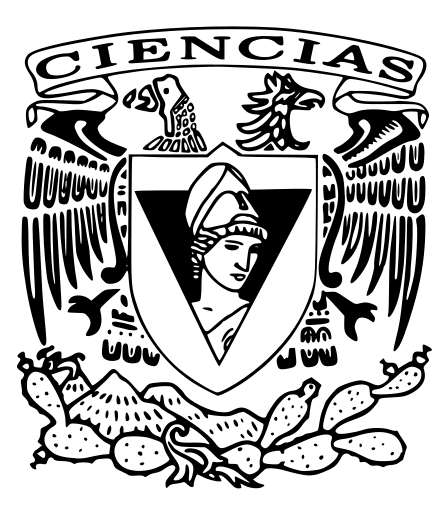
\includegraphics[width=0.5\textwidth]{escudo.png}
		\vfill

		{\large Lunes 26 de octubre del 2018 \par}
	\end{titlepage}

	\pagebreak
	\setlength{\voffset}{-0.75in}
	\setlength{\headsep}{5pt}

	%Ejericios
	\begin{enumerate}
		%1
		\item{
			Suponga de Gage e Itzel participan en un juego, el cual consiste en
			lanzar un dado hasta que alguno de los dos obtenga un 6. Suponga
			que Itzel es la primera en lanzar un dado. ¿Cuál es la probabilidad
			de que Gage gane?
		}

		%2
		\item{
			Considere una variable aleatoria $X$ con una función de densidad
			\[
				f_X(x) = \begin{cases}
					\frac{1-|\frac{x-\alpha}{\beta}|}{\beta},
					$ si $ x \in (\alpha - \beta, \alpha + \beta)\\
					0, $ en otro caso$
				\end{cases}
			\]
			Prueve que $f_X(x)$ es de densidad. Grafíquela.
		}

		%3
		\item{
			\textit{(La paradoja de San Petersburgo, planteada por Nicolás
			Bernoulli en 1728)}.\\
			De acuerdo a la historia, en casino de SanPetersburgo estaba
			dispuesto a ofrecer cualquier tipo de juego siempre que la
			dirección del casino pudiera establecer el precio de la entrara
			que se paga por participar. Se propone el siguiente juego: suponga
			que alguien lanza una moneda balanceada y se reciben $2^n$ pesos
			si cae cara en el $n-$ésimo lanzamiento.\\
			Sea $X$ la ganancia del jugador.
			\begin{enumerate}
				%a
				\item {
				Calcule $\mathbb{E}(X)$.
				}

				%b
				\item {
				¿Estaría dispuesto a liquidar toda la fortuna material que
				posee a cambio de la entrada de este juego?
				}
			\end{enumerate}
		}

		%4
		\item{
			Suponga que se lanzan $n$ dados. Sea $S_n$ la suma de las caras
			obtenidaas al lanzar los $n$ dados.
			\begin{enumerate}
				%a
				\item {
					Encuentre $\mathbb{E}(S_2)$
				}

				%b
				\item {
					Encuentre $\mathbb{E}(S_n)$
				}
			\end{enumerate}
		}

		%5
		\item{
			Sea $Y$ una variable aleatoria con media $\mu > 0$ y varianza
			$\sigma^2 > 0$. Para que valor de $a > 0$ se minimiza
			\begin{enumerate}
				%a
				\item {
					$\mathbb{E}((Y-a)^n)$
				}

				%b
				\item {
					$\mathbb{E}((aY-\frac{1}{a})^2)$
				}
			\end{enumerate}
		}

		%6
		\item{
			Sea $X$ una variable aleatoria con función de densidad
			\[f_X(x) = c \Big(\frac{}{}\Big)^n \mathbb{I}_{\mathbb{N}}(x)\]
			\begin{enumerate}
				%a
				\item {
					Determinar el valor de $c$ para que $f_X$ sea función de
					densidad.
				}

				%b
				\item {
					Encontrar la función generador de momentos $m_X(t)$.
				}
			\end{enumerate}
		}

		%7
		\item{
			Sea $X$ una función de densidad de probabilidad dada por
			\[f_X(x) = \frac{2}{3^x} \mathbb{I}_{\{1, 2, 3, ...\}}(x)\]
			¿Cuál es la probabilidad de que $X$ sea par?
		}

		%8
		\item{
			Sea $X$ variable aleatoria con función de densidad dada por
			\[f_X(x) = \frac{e^{-\frac{x}{2}}}{2}\]
			Con $x > 0$.\\
			Encuentre
			\begin{enumerate}
				%a
				\item {
					$M_X(t)$
				}

				%b
				\item {
					$\mathbb{E}(X)$
				}

				%c
				\item {
					$Var(X)$
				}
			\end{enumerate}
		}

		%9
		\item{
			Demostrar que si $m_X(t)$ es la función generadora de momentos de
			una variable aleatoria $X$, entonces
			\begin{enumerate}
				%a
				\item {
				$\frac{d}{dt}Ln(m_X(t))|_{t = 0} = \mathbb{E}(X)$
				\begin{align*}
					\frac{d}{dt}Ln(m_X(0)) &= \frac{1}{m_X(0)} \cdot m'_X(0)\\
					&= \frac{m'_X(0)}{m_X(0)} = \frac{E(X)}{E(X^0)}\\
					&= E(X)
				\end{align*}
				}

				%b
				\item {
				$\frac{d^2}{dt^2}Ln(m_X(t))|_{t = 0} = Var(X)$
				\begin{align*}
					\frac{d^2}{dt^2}Ln(m_X(0)) &= \frac{d}{dt}\frac{m'_X(0)}{m_X(0)}\\
					&= \frac{m''_X(0)m_X(0)-m'_X(0)m'_X(0)}{m_X(0)^2}\\
					&= \frac{E(X^2) \cdot E(X^0) - E(X)E(X)}{E(X^0)}\\
					&= \frac{E(X^2)-E(X)^2}{1} = E(X^2)-E(X)^2 \\
					&= Var(X)
				\end{align*}
				}
			\end{enumerate}
		}

		%10
		\item{
			Conteste
			\begin{enumerate}
				%a
				\item {
					Si $X$ es una variable aleatoria tal que
					$\mathbb{E}(X) = 3$ y $\mathbb{E}(X^2) = 13$, use la
					desigualdad de Chebyshev para determinar una cota inferior
					para $\mathbb{P}(-2 < X < 8)$.\\
					Notemos que si no sucede que $-2 < X < 8$, entonces  sucede que
					$X \leq -2$ o que $8 \leq X$.\\
					De estas dos ecuaciones tenemos que
					\[X \leq -2 \implies X - 3 \leq -5 \implies -(X - 3) \geq 5\]
					\[ 8 \leq X \implies X - 3 \geq 5\]
					Lo que implica que $|X-3| \geq 5$.\\
					Entonces $-2 < X < 8$ y $|X-3| \geq 5$ son eventos
					complementarios, por lo que
					\[\mathbb{P}(-2 < X < 8) = 1 - \mathbb{P}(|X-3| \geq 5)\]
					Luego, por la desigualdad de Chebyshev,
					\[\mathbb{P}(|X-E(X)| \geq k\sigma) \leq \frac{1}{k^2}\]
					Y se sabe que
					\[E(X) = 3\]
					\[\sigma ^2 = E(X^2) - E(X)^2 = 13 - 9 = 4 \implies \sigma = 2\]
					Entonces
					\[\mathbb{P}(|X-3| \geq 5) = \mathbb{P}(|X-3| \geq 2\cdot \frac{5}{2})
					 \leq \frac{1}{(\frac{5}{2})^2} = \frac{4}{25}\]
					Por lo tanto
					\[\mathbb{P}(-2 < X < 8) = 1 - \mathbb{P}(|X-3| \geq 5)
					\geq 1 - \frac{4}{25} = \frac{21}{25}\]
					Por lo que $\frac{21}{25}$ es una cota inferior de
					$\mathbb{P}(-2 < X < 8)$.
				}

				%b
				\item {
					Sea $X$ una variable aleatoria con función de densidad
					\[
					f_X(x) = \frac{1}{8}\mathbb{I}_{\{-1\}} +
					\frac{6}{8}\mathbb{I}_{\{0\}} +
					\frac{1}{8}\mathbb{I}_{\{1\}}
					\]
					Para $k = 2$, evaluar
					$\mathbb{P}(|X-\mu_X| \geq k\sigma_X)$. Con
					$\mu_X = \mathbb{E}(X)$. Compare con la cota dada por la
					desigualdad de Chebyshev.
					\[\mathbb{E}(X) = \sum{x_i f_X(x_i)} = -1\frac{1}{8}
					+ 0 \frac{6}{8} + 1 \frac{1}{8} = 0\]
					\[\mathbb{E}(X^2) = \sum{(x_i)^2 f_X(x_i)} = 1\frac{1}{8}
					+ 0 \frac{6}{8} + 1 \frac{1}{8} = \frac{1}{4}\]
					\[\sigma_X = E(X^2) - E(X)^2 = \frac{1}{4} - (0)^2 = \frac{1}{4}\]
					Por lo que
					\[\mathbb{P}(|X-\mu_X| \geq k\sigma_X)) =
					\mathbb{P}(|X| \geq 2 \cdot \frac{1}{4})
					= \mathbb{P}((X \geq \frac{1}{2}) \cup (X \leq -\frac{1}{2}))\]
					Y como $X \geq \frac{1}{2}$ y $X \leq -\frac{1}{2}$ no
					pueden pasar al mismo tiempo, son ajenos, por lo que
					\begin{align*}
						\mathbb{P}((X \geq \frac{1}{2}) \cup (X \leq -\frac{1}{2}))
						&= \mathbb{P}(X \geq \frac{1}{2})
						+ \mathbb{P}(X \leq -\frac{1}{2})\\
						&= \frac{1}{8} + \frac{1}{8} = \frac{1}{4}
					\end{align*}
					Por otra parte, por la desigualdad de Chebyshev.
					\[\mathbb{P}(|X-0| \geq 2 \cdot \frac{1}{4}) \leq \frac{1}{2^2}
					= \frac{1}{4} \]
					Por lo que el valor real y la cota obtenida por la
					desigualdad de Chebyshev son iguales.
				}

				%c
				\item {
					Suponga que $X$ es una variable aleatoria con media y
					varianza igual a 20. ¿Qué se puede decir de
					$\mathbb{P}(0 \leq X \leq 40)$?\\
					El evento contrario sería que $X < 0$ o $40 < X$. De aquí
					\begin{align*}
						X < 0 &\implies X - 20 < -20 \implies -(X-20) > 20\\
						40 < X &\implies X - 20 > 20\\
						\implies &|X-20|>20
					\end{align*}
					Entonces, $P(0 \leq X \leq 40) = 1 - P(|X-20|>20)$.\\
					Luego, por la desigualdad Chebyshev,
					\[P(|X-E(X)| > k\sigma) < \frac{1}{k^2}\]
					Como $E(X) = \sigma ^2 = 20$, entonces $k=\sqrt{20}$.
					Por lo que
					\[P(|X-20| > 20)  = P(|X-20| > \sqrt{20}\sqrt{20}) <
					\frac{1}{20}\]
					Finalmente
					\[P(0 \leq X \leq 40) = 1 - P(|X-20| > 20)
					> 1 - \frac{1}{20} = \frac{19}{20}\]
					Se puede decir que $P(0 \leq X \leq 40)$ es mayor a
					$\frac{19}{20}$.
				}
			\end{enumerate}
		}

		%11
		\item{
			Si $X$ es una variable aleatoria tal que $\mathbb{E}(X) = 3$ y
			$\mathbb{E}(X^2) = 13$, use la desigualdad de Chebyshev para
			determinar una cota mínima para $\mathbb{P}(-2 < X < 8)$.\\
			Notemos que si no sucede que $-2 < X < 8$, entonces  sucede que
					$X \leq -2$ o que $8 \leq X$.\\
					De estas dos ecuaciones tenemos que
					\[X \leq -2 \implies X - 3 \leq -5 \implies -(X - 3) \geq 5\]
					\[ 8 \leq X \implies X - 3 \geq 5\]
					Lo que implica que $|X-3| \geq 5$.\\
					Entonces $-2 < X < 8$ y $|X-3| \geq 5$ son eventos
					complementarios, por lo que
					\[\mathbb{P}(-2 < X < 8) = 1 - \mathbb{P}(|X-3| \geq 5)\]
					Luego, por la desigualdad de Chebyshev,
					\[\mathbb{P}(|X-E(X)| \geq k\sigma) \leq \frac{1}{k^2}\]
					Y se sabe que
					\[E(X) = 3\]
					\[\sigma ^2 = E(X^2) - E(X)^2 = 13 - 9 = 4 \implies \sigma = 2\]
					Entonces
					\[\mathbb{P}(|X-3| \geq 5) = \mathbb{P}(|X-3| \geq 2\cdot \frac{5}{2})
					 \leq \frac{1}{(\frac{5}{2})^2} = \frac{4}{25}\]
					Por lo tanto
					\[\mathbb{P}(-2 < X < 8) = 1 - \mathbb{P}(|X-3| \geq 5)
					\geq 1 - \frac{4}{25} = \frac{21}{25}\]
					Por lo que $\frac{21}{25}$ es una cota mínima de
					$\mathbb{P}(-2 < X < 8)$.
		}

		%12
		\item{
			Demuestre o dé un contraejemplo
			\begin{enumerate}
				%a
				\item {
					Existe una variable aleatoria $X$ para la cual
					\[\mathbb{P}(\{\omega \in \Omega : E(X) - 2_{\sigma_X} <
					X(\omega) <
					E(X) + 2_{\sigma_X}\}) = \frac{3}{5}\]
				}

				%b
				\item {
					Si $X$ es una variable aleatoria no negativa, entonces
					$\mathbb{E}(X) \leq (\mathbb{E}(X^2))^{\frac{1}{2}}$.
				}
			\end{enumerate}
		}

		%13
		\item{
			Considerese una variable aleatoria $X$ con función de densidad
			$f_X(x) = 2(1-x)\mathbb{I}_{\{0, 1\}}(x)$.\\
			Calcule $\mathbb{E}((X+10)^2)$ y
			$\mathbb{E}\Big(\frac{1}{1-X}\Big)$.
		}

		%14
		\item{
			Un experimento consiste en lanzar dos bolas dentro de cuatro cajas
			de tal forma que cada bola tiene la misma probabilidad de caer en
			cualquier caja. Sea $X$ el número de bolas en la primera caja.
			\begin{enumerate}
				%a
				\item {
					¿Cuál es la función de distribución acumulativa de $X$?
				}

				%b
				\item {
					¿Cuál es la función de densidad de $X$?
				}

				%c
				\item {
					Encontrar $\mathbb{E}(X)$ y $Var(X)$.
				}
			\end{enumerate}
		}

		%15
		\item{
			Sean $a_1, a_2, ..., a_n$ números positivos. Se define
			\begin{align*}
				a_A &= \frac{1}{n}\sum_{i = 0}^{n}{a_i}\\
				a_G &= (\prod_{i = 1}^{n}{a_i})^{\frac{1}{n}}\\
				a_H &= \frac{1}{\frac{1}{n}(\frac{1}{a_1} + ...
				+ \frac{1}{a_n})}
			\end{align*}
			como las medidas aritmética, geométrica y armónica respectivamente.
			Usando la desigualdad de Jenses, demuestre que
			\[a_H \leq a_G \leq a_A\]
			\textit{Demostración}:\\
		    La desigualdad de Jensen nos dice que para el caso finito si f es una función convexa entonces:
			\begin{center}
			    $$f(\frac{\sum a_{i}x_{i}}{\sum a_{i}})\leq \frac{\sum a_{i}f(x_{i})}{\sum a_{i}}$$
			\end{center}
			Y si es una función concava se sigue que:\\
			\begin{center}
			    $$f(\frac{\sum a_{i}x_{i}}{\sum a_{i}})\geq \frac{\sum a_{i}f(x_{i})}{\sum a_{i}}$$
			\end{center}
			Con $\lbrace x_{i} \rbrace _{i=1}^{n}$ elementos del dominio de f y $\lbrace a_{i} \rbrace _{i=1}^{n}$ pesos positivos.\\
		   Tomando a $f(x)=log(x)$ y $a_{i}=1 \ \forall i\in \lbrace 1,...,n \rbrace$ se sigue que por criterio de la segunda derivada con respecto de f(x):\\
		   \begin{center}
		       $f'(x)=\frac{1}{x} \ \ \Rightarrow  f''(x)=-\frac{1}{x^2}$
		   \end{center}
		   Se sigue que $\forall x\in Dom(f)$ $f''(x)$ es negativa  ya que $x^2^$ es positiva siempre. Entonces por criterio de la segunda derivada es concava. Entonces tenemos que usando la desigualdad de Jensen:\\
		   \begin{center}
		       $$log(\frac{\sum_{i=1}^{n} a_{i}x_{i}}{\sum_{i=1}^{n} a_{i}})\geq \frac{\sum_{i=1}^{n} a_{i}log(x_{i})}{\sum_{i=1}^{n} a_{i}}$$
		   \end{center}
		   Pero como $a_{i}=1 \ \forall i$ entonces:
		   \begin{center}
		       $$log(\frac{\sum_{i=1}^{n}x_{i}}{n})\geq \frac{\sum_{i=1}^{n}log(x_{i})}{n}$$
		   \end{center}
		   Pero por propiedades de logaritmo se sigue que:
		   $$\sum_{i=1}^{n}log(x_{i})=log(\prod_{i=1}^{n}x_{i})$$ \\
		      $$\frac{log(x)}{n}=log(x^{\frac{1}{n}})$$\\
		      Entonces:\\
		      \begin{center}
		     $$log(\frac{\sum_{i=1}^{n}x_{i}}{n})\geq log((\prod_{i=1}^{n}x_{i})^{\frac{1}{n}})
		      $$\end{center}
		      Y eso sucede solamente cuando:\\
		      \begin{center}
		          $$a_{A}=\frac{\sum_{i=1}^{n}x_{i}}{n} \geq (\prod_{i=1}^{n}x_{i})^{\frac{1}{n}}=a_{G}$$
		      \end{center}
		      Y eso es igual a decir que $a_{A}\geq a_{G}$. Ahora, podemos reescribir a $a_{H}$ de la siguiente forma:\\
		      \begin{center}
		          $$\frac{1}{(\frac{1}{n})(\sum_{i=1}^{n}(\frac{1}{a_{i}}))}=\frac{n}{\sum_{i=1}^{n}(a_{i})^{-1}}=(\frac{\sum_{i=1}^{n}(a_{i})^{-1}}{n})^{-1}$$
		      \end{center}
		      Reescribiendo a $(a_{i})^{-1}=k_{i}$ por la desigualdad antes vista se tiene que:\\
		      \begin{center}
		          $$\frac{\sum_{i=1}^{n}k_{i}}{n}\geq (\prod_{i=1}^{n}k_{i})^{\frac{1}{n}}$$
		      \end{center}
		      Por propiedades de producto, el exponente se distribuye de la siguiente manera:\\
		      \begin{center}
		          $$\frac{\sum_{i=1}^{n}k_{i}}{n}\geq \prod_{i=1}^{n}(k_{i})^{\frac{1}{n}}$$
		      \end{center}
		      Y reemplazando $k_{i}$ por $a_{i}^{-1}$\\
		      \begin{center}
		          $$\frac{\sum_{i=1}^{n}(a_{i})^{-1}}{n} \geq \prod_{i=1}^{n}a_{i}^{-\frac{1}{n}}$$
		      \end{center}
		      Y por las mismas propiedades de exponentes se tiene que:\\
		      \begin{center}
		          $$\frac{\sum_{i=1}^{n}(a_{i})^{-1}}{n}\geq (\prod_{i=1}^{n}(a_{i})^{\frac{1}{n}})^{-1}$$
		      \end{center}

		      Entonces se tiene que:\\
		      \begin{center}
		          $$\frac{\sum_{i=1}^{n}(a_{i})^{-1}}{n}\geq \frac{1}{(\prod_{i=1}^{n}a_{i})^{\frac{1}{n}}}$$\\ \\
		          $$a_{G}=(\prod_{i=1}^{n}a_{i})^{\frac{1}{n}}\geq \frac{n}{\sum_{i=1}^{n}(a_{i})^{-1}}=\frac{1}{\frac{1}{n}(\sum_{i=1}^{n}(\frac{1}{a_{i}}))}=a_{H}$$

		      \end{center}
		      Entonces $a_{G}\geq a_{H}$ pero $a_{A}\geq a_{G}$ entonces:\\
		      \begin{center}
		          $$a_{A}\geq a_{G} \geq a_{H}_{\blacksquare}$$
		      \end{center}

 		}

		%16
		\item{
			Sea $X$ una variable aleatoria no negativa con media 25. ¿Qué puede
			decir de las siguientes cantidades?
			\begin{enumerate}
				%a
				\item {
					$\mathbb{E}(X^3)$ \\

				Tenemos que $\frac{d^2}{dx^2}x^3=6x$ y como X es variable aleatoria no negativa tenemos que $6x>0 \ \forall x$. Entonces es una función convexa entonces se cumple que:\\
				\begin{center}
				    $E(X)^3 \leq E(X^3)$
				\end{center}
				Pero como $E(X)=25$ entonces:\\
				\begin{center}
				    $E(X)< E(X^3)$
				\end{center}

				}


				%b
				\item {
					$\mathbb{E}(\sqrt{X})$

				Tenemos que si $f(x)=\sqrt{x}$ se sigue que $f''(x)=-\frac{1}{4\sqrt{x^3}}$ y como $x>0 \ \forall x\in Dom(f)$ porque nuestra variable aleatoria es positiva se sigue entonces que $f''(x)<0$ entonces es concava entonces:\\
				\begin{center}
				    $\sqrt{E(X)}\geq E(\sqrt{X})$
				\end{center}
				Pero, como $E(X)=25 \ \Rightarrow \sqrt{E(X)}=5$ entonces:\\
				\begin{center}
				    $E(X) > E(\sqrt{X})$
				\end{center}

				}

				%c
				\item {
					$\mathbb{E}(log(X))$\\ \\
					Como $log(x)$ es una función cóncava (inciso anterior) entonces por la desigualdad de Jensen para la esperanza se sigue que:\\
					\begin{center}
					    $log(E(X))\geq E(log(X))$
					\end{center}
					Y por propiedades de logaritmo: $log(x)\leq x-1 \ \Rightarrow log(x) < x$ entonces:\\
					\begin{center}
					    $E(X)> log(E(X)) \geq E(log(X)) \Rightarrow E(X) > E(log(X))$
					\end{center}
				}

				%d
				\item {
					$\mathbb{E}(e^{-X})$\\
					Tenemos que:\\
					\begin{center}
					    $$\frac{d^2}{dx^2} e^{-x}=e^{-x}=\frac{1}{e^x}$$
					\end{center}
					Tenemos que como $\frac{1}{e^x}>0 \ \forall x\in Dom(f)$ la función es convexa. Entonces por desigualdad de Jensen:\\
					\begin{center}
					    $e^{-E(X)}\leq E(e^{-x})$
					\end{center}
					Pero $E(X)=25$ entonces:\\
					\begin{center}
					    $$\frac{1}{e^{25}}\leq E(e^{-x})$$
					\end{center}
				}
			\end{enumerate}
		}

		%17
		\item{
			\textbf{(OPCIONAL)}\\
			Si $X$ es una variable aleatoria con valor esperado finito,
			entonces
			\[\mathbb{E}(X) = \int_{0}^{\infty}{(1-F_X(x))dx} -
			\int_{-\infty}^{0}{F_X(x)dx}\]


			\begin{align*}
E[X] &= E\bigg[\int_0^X 1\,dx\bigg]\\
&= E\bigg[\int_0^\infty 1_{\{X>x\}}\,dx\bigg]\\
&= \int_0^\infty E[1_{\{X>x\}}]\,dx\\
&= \int_0^\infty P(X > x)\,dx\\
&= \int_0^\infty (1 - F(x))\,dx
\end{align*}

		}

	\end{enumerate}
\end{document}
